%%%%%%%%%%%%%%%%%%%%%%%%%%%%%%%%%%%%%%%%%%%%%%%%%%%%%%%%%%%%%%%%%%%%%%%%%%%
%%%                         Projeto                                 %%%
%%%%%%%%%%%%%%%%%%%%%%%%%%%%%%%%%%%%%%%%%%%%%%%%%%%%%%%%%%%%%%%%%%%%%%%%%%%

\chapter{Projeto}
\label{ch:projeto}
Diante do cenário exposto na introdução e fundamentação teórica, evidencia-se a
necessidade de estratégias pedagógicas que fortaleçam o ensino de matemática,
especialmente no que se refere ao engajamento dos estudantese o desenvolvimento
de habilidades para resolução de problemas dos alunos.

O sistema Cognitivo é um ambiente gamificado focado no engajamento para
a disciplina de matemática no contexto da prova do ENEM, utilizando como base
estrutural os quatro pilares do PC. A plataforma foca na resolução de problemas
em níveis que seguem os conceitos de decomposição, reconhecimento de padrões,
abstração e algoritmos.

\section{Diagrama de Caso de Uso}
O Diagrama de caso uso abaixo retrata o comportamento funcional do sistema 
sob a perspectiva das interações com os usuários. 

\begin{figure}[H]
    \centering
    \caption{Diagrama de Caso de Uso}
    \label{fig:diagrama-caso-uso}
    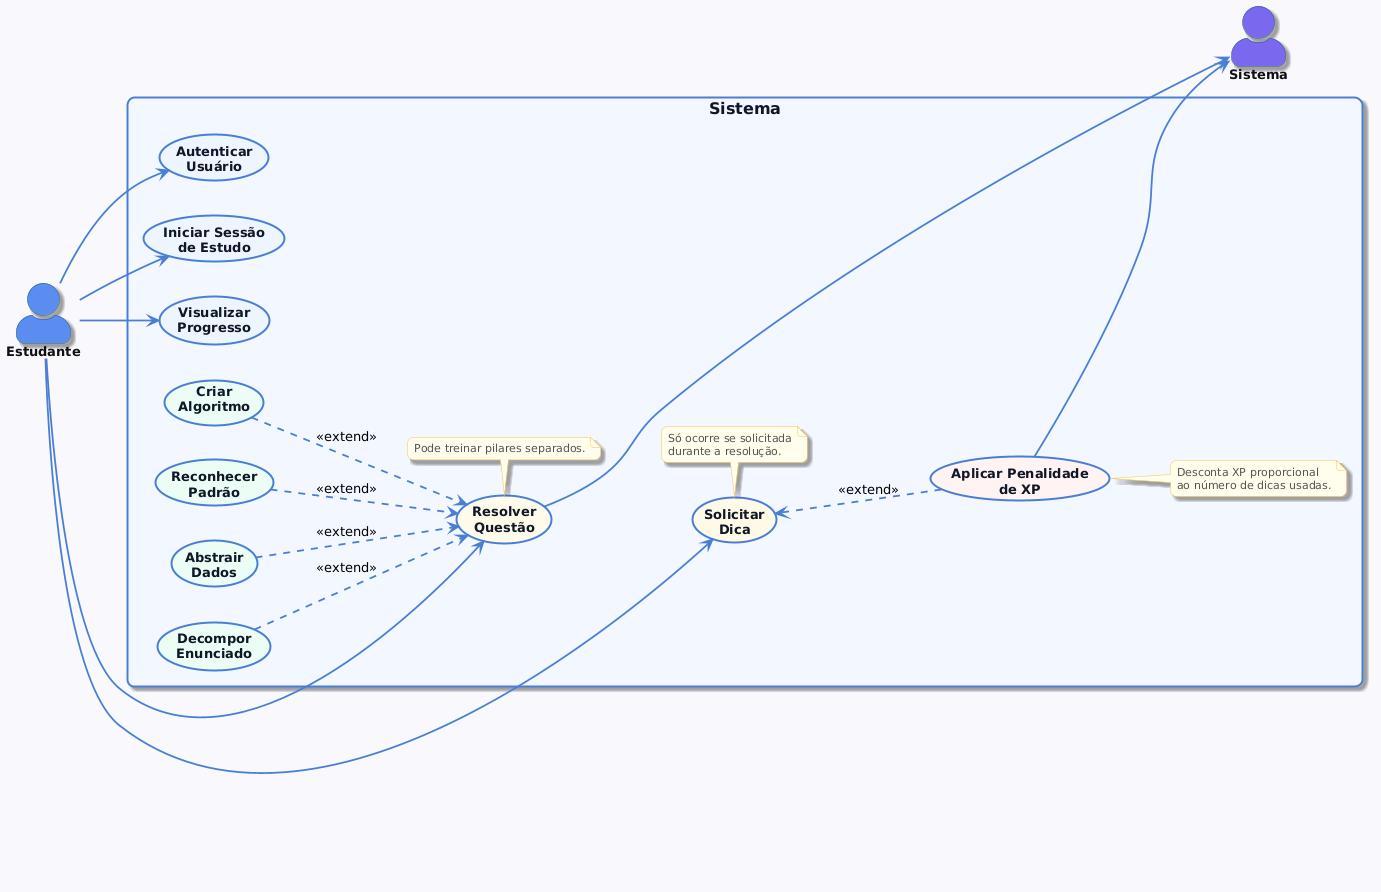
\includegraphics[width=\textwidth]{figuras/Diagrma_de_Caso_De_Uso.png}
    \fonte{Elaborado pelo autor (2026).}
\end{figure}

O ator Estudante relaciona-se com os casos de uso de Autenticar Usuário,
responsável por gerenciar o controle de acesso, e Iniciar Sessão de Estudo, que
estabelece o início de uma nova trilha de exercícios.

Visualizar Progresso, funcionalidade que renderiza estatísticas de uso na
plataforma: nível, posição na liga global, \textit{badges}, sequência de dias
ativos e níveis de engajamento por assuntos.

O núcleo da plataforma é centralizado no caso de uso Resolver Questão. O sistema
guia o aluno pelas fases Abstrair Dados, Decompor Enunciado, Reconhecer Padrão e
Criar Algoritmo. O estudante pode treinar cada pilar separado, por isso a
relação \textit{extend}. 

O Estudante pode acionar o caso de uso Solicitar Dica quando encontrar
dificuldades em cada nível. Com o erro, o sistema calcula de forma proporcional
a penalidade via caso de uso Aplicar Penalidade XP.


\section{Arquitetura do Sistema}
Segundo \cite{brown_c4_model_book}, a arquitetura de um Sistema de Software é
uma estrutura composta por contêineres. Esses Contêineres consistem em diversas
aplicações e armazenamentos de dados que, juntos, integram o sistema, englobando
esquemas de banco de dados, aplicativos móveis, aplicações de console e
aplicações web executadas tanto no lado do servidor quanto no cliente. 

\begin{figure}[H]
    \centering
    \caption{Diagrama de Arquitetura}
    \label{fig:diagrama-arquitetura}
    
\includegraphics[width=0.95\textwidth]{diagrama_arquitetura.png}
    \fonte{Elaborado pelo autor (2026).}
\end{figure}

\subsection{Módulo ETL}

Segundo, \cite{kimball2004data} o \textit{Extract, Transform, Load} (ETL) é o
sistema de fluxo contínuo que, inicialmente, extrai as informações dos sistemas
de origem, processo e realiza a limpeza dos dados ao estabelecer padrões de
qualidade e consistência, englobando a remoção de erros, a correção de dados
faltantes e a disponibilização de métricas documentadas que atestam a
confiabilidade dessas informações.

O módulo ETL inicia o fluxo de dados pelo contêiner de Extração com
rotinas em \textit{Python} usando as bibliotecas \textit{requests} e
\textit{httpx} para coletas em lote com \textit{self-hosted} da
\href{https://enem.dev/}{API ENEM DEV}, evitando limitações impostas por
terceiros. 

A biblioteca \textit{requests} executa chamadas síncronas para
consultas estruturais pontuais na instância \textit{self-hosted} da API. A
biblioteca \textit{httpx} implementa o processamento assíncrono para a coleta
massiva de dados. Esse mecanismo permite requisições de questões simultaneamente
sem aguardar a resposta de cada chamada anterior.

Os dados brutos são encaminhados para o container de Transformação, no qual
scripts em \textit{Python} usando bibliotecas como \textit{Pandas} e
\textit{Pydantic} realizam a normalização, validação e o enriquecimento das
informações. Essas bibliotecas, respectivamente, permitem organizar as
informações em uma estrutura de tabela, limpar textos com erros de formatação,
tratar caracteres corrompidos e erros de formatação das questões e outras atividades 
de tratamento e normalização de dados.

O enriquecimento consiste em mapear e estruturar cada questão do ENEM de acordo
com os pilares do PC. O processo associa o enunciado e a resolução da questão
aos conceitos de decomposição, reconhecimento de padrões, abstração e
algoritmos.

Os dados são armazenados no \textit{PostgreSQL} que atua como área de staging,
pois, de acordo com \cite{kimball2004data}, a gravação dos dados em disco em
formatos permanentes ou semipermanentes ao longo das diversas etapas do fluxo
garante a integridade e o rastreamento do processo.

\subsection{Sistema Gamificado}
O estudante acessa via protocolo \textit{HyperText Transfer Protocol Secure (HTTPS)}
por meio de seu navegador com a aplicação web. 

O \textit{React} gerencia o estado da aplicação, permitindo que as transições
entre os níveis (pilares do PC) ocorram de forma fluida e sem a necessidade de
recarregar a página. O \textit{Tailwind CSS} fornece classes utilitárias que
garantem a total responsividade do layout, adaptando o jogo para
dispositivos \textit{desktop} e \textit{mobile}.

A camada de comunicação entre o front-end em \textit{React} e a \textit{API
Gateway} em \textit{FastAPI} baseia-se no modelo cliente-servidor. O
\textit{FastAPI} atua como o ponto de entrada, recebendo todas as requisições
oriundas do cliente e encaminhar em formato \textit{JavaScript Object Notation (JSON)} para o motor pedagógico.

Uma vez validados, os dados fluem para o Motor Pedagógico e de
Gamificação, back-end da aplicação, implementado em \textit{Python} que
centraliza as regras de negócio do sistema. 

Para garantir a persistência e a recuperação dos dados de progresso e usuários,
este motor se comunica com o Banco de Dados Relacional \textit{MySQL}.

As tabelas abaixo retratam aspectos da gamicação implementada na aplicação

\begin{table}[htbp]

    \centering
  \caption{\label{table:pontos_xp}Distribuição de pontos de experiência (XP) por etapa concluída}

  \begin{tabular}{|l|c|c|} % O uso das barras '|' cria as linhas verticais exigidas para quadros

  \hline

  \textbf{Etapa concluída} & \textbf{XP geral (Float)} & \textbf{XP de atributo (Float)} \\ \hline

  Decomposição & +2.0 & +2.0 \\ \hline

  Abstração & +2.0 & +2.0 \\ \hline

  Padrões & +2.0 & +2.0 \\ \hline

  Algoritmos & +3.0 & +3.0 \\ \hline

  Conclusão (Bônus) & +1.0 & +0.25 (em cada atributo) \\ \hline

  \end{tabular}

  \fonte{Elaborada pelo autor (2026).}

\end{table}


\begin{table}[htbp]

  \centering

  \caption{\label{table:penalidades_xp}Matriz de penalidades}

  \begin{tabular}{|l|c|c|}

  \hline

  \textbf{Ação do usuário} & \textbf{Penalidade} & \textbf{Impacto no XP} \\ \hline

  Tentativa errada & $\times 0.98$ ($-2\%$) & Mínimo \\ \hline

  Erro persistente (3+) & $\times 0.90$ ($-10\%$) & Leve \\ \hline

  Dica 1 & $\times 0.80$ ($-20\%$) & Médio \\ \hline

  Dica 2 & $\times 0.50$ ($-50\%$) & Alto \\ \hline

  Dica 3 & $\times 0.40$ ($-60\%$) & Crítico \\ \hline

  \end{tabular}

  \fonte{Elaborada pelo autor (2026).}

\end{table}

\section{Design}
O design da aplicação é fundamentado em princípios de usabilidade,
acessibilidade e engajamento, visando proporcionar uma experiência intuitiva e
motivadora para os estudantes. A interface é projetada para ser limpa e
organizada, com uma paleta de cores que favorece a leitura e a concentração.

De acordo com \cite{preece2013design}, o design deve ser implementado com uma
preocupação central em desenvolver produtos interativos que sejam utilizáveis,
sendo fáceis de aprender, eficazes no uso. É proporcionar uma experiência
agradável.

A interface da aplicação é desenvolvida com foco na simplicidade e na clareza,
utilizando uma estrutura de navegação intuitiva. Os elementos visuais são
organizados de maneira a guiar o usuário através das diferentes etapas do
processo de resolução de problemas, destacando as mecânicas de gamificação para
incentivar o engajamento. Esse processo busca atender as metas de usabilidade. É
descrito por \cite{preece2013design}, para ser eficaz, eficiente, segura no uso,
boa utlidade, fácil de aprender e fácil de lembrar.

Segundo \cite{preece2013design} eficácia é quanto um sistema é bom no que se
propõe. A eficiência refere-se como o sistema auxilia o usuário a realizar suas
tarefas com o mínimo de esforço. A segurança no uso é a capacidade do sistema de
prevenir erros e minimizar as consequências de erros inevitáveis. A boa
utilidade é a capacidade do sistema de fornecer as funcionalidades necessárias
para os usuários alcançarem seus objetivos. A facilidade de aprendizado é a
rapidez com que os usuários podem aprender a usar o sistema. A facilidade de
lembrar é a capacidade do sistema de permitir que os usuários se lembrem de como
usá-lo após um período de não uso .

O fluxo de navegabilidade abaixo retrata a sequência de passos feitas pelo
usuário no sistema e será validado nos cilcos iterativos descritos
anteriormente.
\begin{figure}[H]
    \centering
    \caption{Fluxo de navegabilidade}
    \label{fig:design}
    \includegraphics[width=0.95\textwidth]{figuras/Fluxo de navegabilidade Final.png}
    \fonte{Elaborado pelo autor (2026).}
\end{figure}

